\documentclass[xcolor=x11names,compress]{beamer}
\usepackage[utf8]{inputenc}
\usepackage[spanish]{babel}
\usepackage{hyperref}
\hypersetup{colorlinks=true,linkcolor=black}
\usepackage{colortbl}
\usepackage{xcolor}
\usepackage{multirow}
\usepackage{fancyhdr}
\usepackage{graphicx}
\usepackage{framed}
\usepackage[version=0.96]{pgf}
\usepackage{listings}

\usepackage{changepage}
\usepackage{lipsum}
\usepackage{multicol}


\lstdefinelanguage{JavaScript}{
  keywords={typeof, new, true, false, catch, function, return, null, catch, switch, var, if, in, while, do, else, case, break},
  keywordstyle=\color{blue}\bfseries,
  ndkeywords={class, export, boolean, throw, implements, import, this},
  ndkeywordstyle=\color{darkgray}\bfseries,
  identifierstyle=\color{black},
  sensitive=false,
  comment=[l]{//},
  morecomment=[s]{/*}{*/},
  commentstyle=\color{purple}\ttfamily,
  stringstyle=\color{red}\ttfamily,
  morestring=[b]',
  morestring=[b]"
}


\definecolor{shadecolor}{RGB}{243,243,243}
\renewcommand{\figurename}{Figura}

\newtheoremstyle{cuadrado}% name
  {1pt}%      Space above
  {8pt}%      Space below
  {\itshape}%         Body font
  {}%         Indent amount (empty = no indent, \parindent = para indent)
  {\itshape}% Thm head font
  {}%        Punctuation after thm head
  {0em}%     Space after thm head: " " = normal interword space;
        %       \newline = linebreak
  {}%         Thm head spec (can be left empty, meaning `normal')

\theoremstyle{cuadrado}
\newtheorem*{teo}{}

\newcommand{\slidesettitulo}{\textcolor{black}{Multi Sensor Robot System (SensorRS), Vehículo
robótico multisensorial de exploración controlado por
wifi basado en Arduino y Raspberry Pi}}
\newcommand{\shorttitulo}{SensorRS}
\newcommand{\email}{{
\includegraphics[width=2.5cm]{logotipo.png}}}
\newcommand{\web}{}
\newcommand{\institucion}{Universidad de Cádiz  \\ Escuela Superior de Ingeniería \\ \vspace*{1ex} MÁSTER UNIVERSITARIO EN INVESTIGACIÓN EN
INGENIERÍA DE SISTEMAS Y DE LA COMPUTACIÓN }

\newcommand{\authornombre}{Manuel López Urbina \vspace*{1ex}}
\newcommand{\tutor}{Arturo Morgado Estévez}
\newenvironment{fondo}{\begin{teo}}{\end{teo}}

\definecolor{darkgray}{RGB}{237,236,236}
\definecolor{azuladwys}{RGB}{157,189,219}
\definecolor{azuladwys_version}{RGB}{174,208,239}
\definecolor{plata}{RGB}{145,143,144}


\usetheme{Ilmenau}

\setbeamertemplate{footline}{
\begin{tiny}
\setbeamercolor{foot1}{fg=black!70,bg=gray!10}
\setbeamercolor{foot2}{fg=gray,bg=gray!15}
\setbeamercolor{foot3}{fg=gray,bg=gray!10}
\setbeamercolor{foot4}{fg=black!70,bg=gray!20}
\setbeamercolor{foot5}{fg=gray,bg=gray!15}
\setbeamercolor{foot6}{fg=black,bg=gray!20}

%\setbeamercolor{foot1}{fg=azuladwys_version,bg=azuladwys_version}
%\setbeamercolor{foot2}{fg=azuladwys,bg=azuladwys}
%\setbeamercolor{foot3}{fg=azuladwys_version,bg=azuladwys_version}
%\setbeamercolor{foot4}{fg=azuladwys,bg=azuladwys}
%\setbeamercolor{foot5}{fg=azuladwys,bg=azuladwys}
%\setbeamercolor{foot6}{fg=black,bg=gray!20}

% taken from theme infolines and adapted
  \leavevmode%
  \hbox{%
  \begin{beamercolorbox}[wd=.35\paperwidth,ht=2.25ex,dp=1ex,center]{foot1}%
  %\fontsize{5}{5}\selectfont
  \shorttitulo
  \end{beamercolorbox}%
  \begin{beamercolorbox}[wd=.1\paperwidth,ht=2.25ex,dp=1ex,center]{foot2}
  \end{beamercolorbox}%
    \begin{beamercolorbox}[wd=.05\paperwidth,ht=2.25ex,dp=1ex,center]{foot3}
  \end{beamercolorbox}%
    \begin{beamercolorbox}[wd=.25\paperwidth,ht=2.25ex,dp=1ex,center]{foot4}%
  %\fontsize{5}{5}\selectfont
  \web
  \end{beamercolorbox}%
  \begin{beamercolorbox}[wd=.05\paperwidth,ht=2.25ex,dp=1ex,center]{foot5}
  \end{beamercolorbox}%
  \begin{beamercolorbox}[wd=.2\paperwidth,ht=2.25ex,dp=1ex,right]{foot6}%
	\insertframenumber{} / \inserttotalframenumber \hspace*{2ex} 
  \end{beamercolorbox}}%
  \vskip0pt%
\end{tiny}
\vskip10pt
}


%\setbeamertemplate{footline}{}
\setbeamertemplate{navigation symbols}{} %Elimina los iconos que permiten la navegación en el documento

\usecolortheme[named=darkgray]{structure}
\usefonttheme{professionalfonts}
\useoutertheme{miniframes}

\title{\slidesettitulo}
\author{\authornombre \\ \email \\ Director: \tutor}
\institute{\institucion}
\date{ }
\setcounter{subsection}{0}



\begin{document}
\scriptsize{

\frame{\titlepage}

%\section{Índice}
%\frame{\frametitle{\textcolor{black}{Índice}}
%  \textcolor{black}{\tableofcontents}
%}


\section{Índice}

\begin{frame}{\contentsname}
\begin{multicols}{2}
  \textcolor{black}{\tableofcontents}
\end{multicols}
\end{frame}


\section{Objetivos}

\frame{\frametitle{\textcolor{black}{ Objetivos }}

SensorRS es un proyecto robótico elaborado principalmente con una placa Raspberry Pi interconectada por puerto serie
con una placa Arduino.\\

\begin{itemize}
 \item Sistema dotado de multitud de sensores para captar información del entorno en el que el robot se encuentra.
 \item Destinado al área de la exploración reduciendo la exposición de personas en zonas peligrosas.
 \item Sistema basado una arquitectura en microcontroladores programables, mayor ecalabilidad, incorporación de más sensores, etc. 
\end{itemize}

\begin{figure}[H]
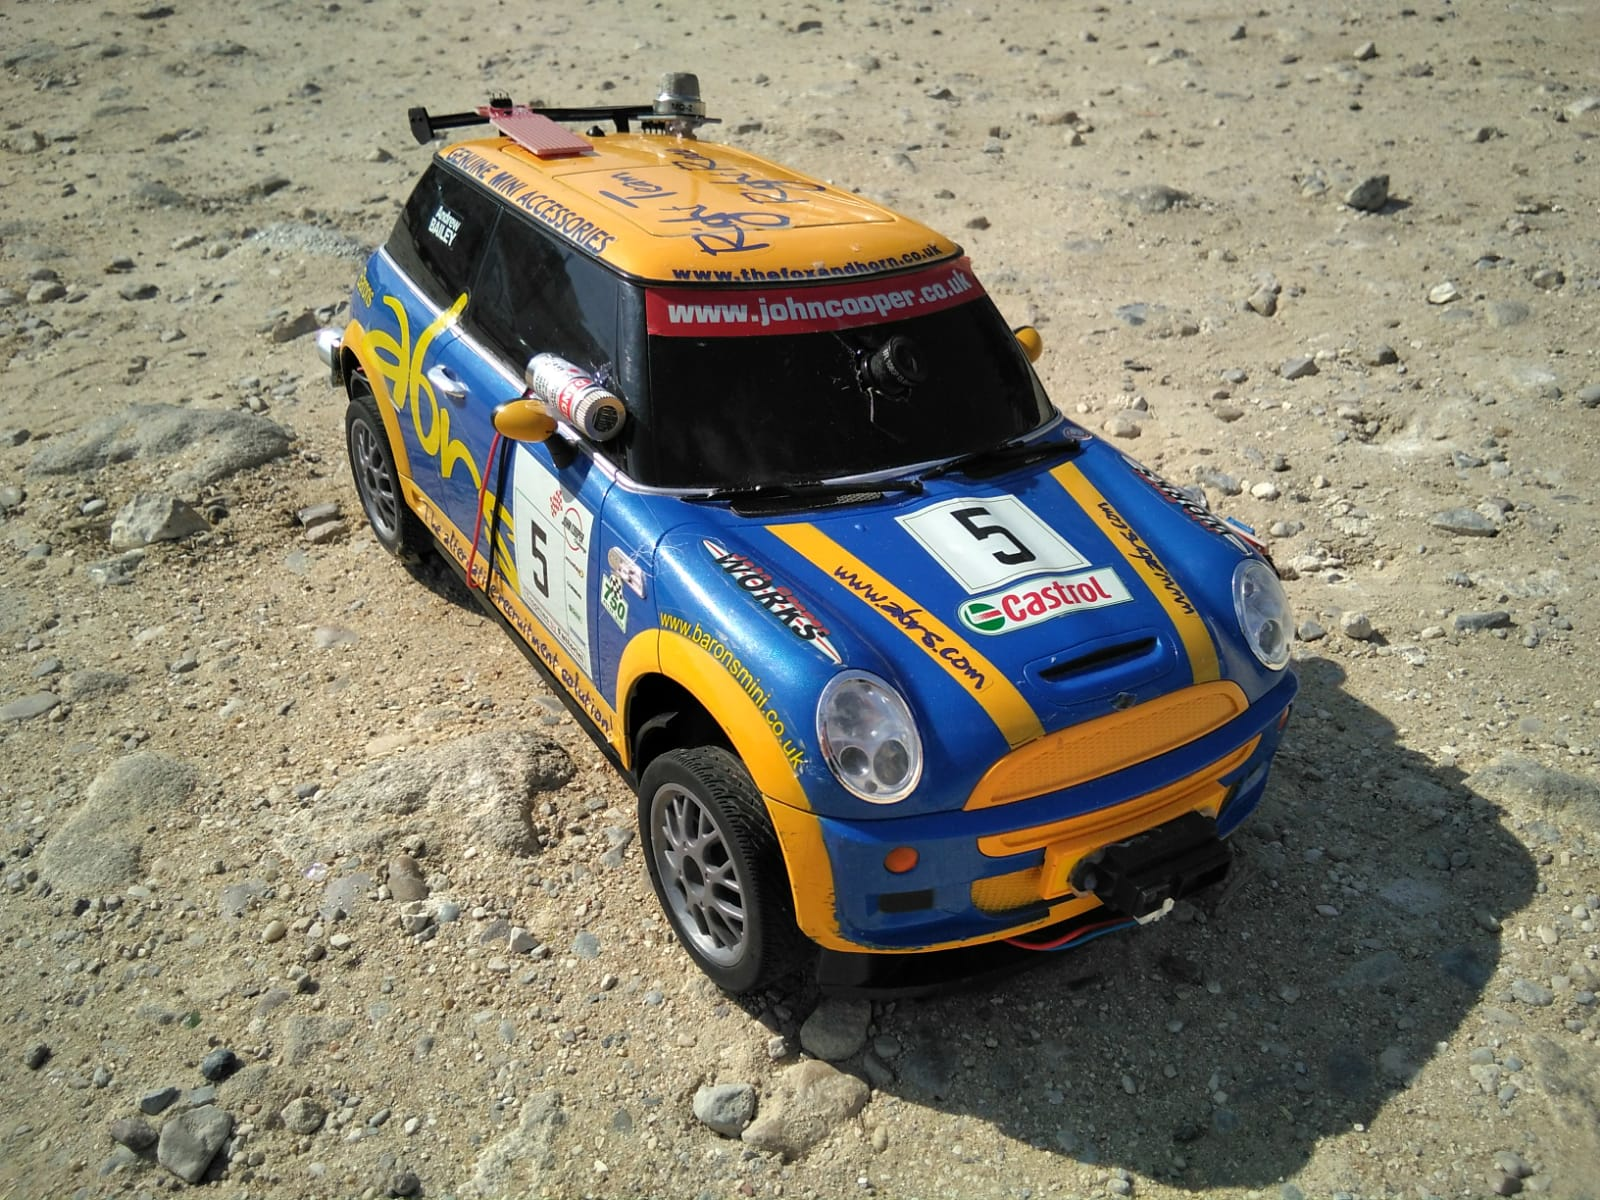
\includegraphics[width=4cm]{tierra.jpg}
\end{figure}

\begin{center}
 \fontsize{20pt}{12pt}\selectfont
 \emph{Vehículo SensorRS}
\end{center}

}

\section{Alcance}

\frame{\frametitle{\textcolor{black}{ Alcance }}

\begin{columns}
\begin{column}{0.5\textwidth}

\begin{itemize}
 \item Sistema basado en Raspberry Pi gobernada vía wifi a través de la aplicación web RobotUI constituyendo éste el nivel superior del sistema.
 \item Placa Arduino gestionada por Raspberry Pi encargada del control de sensores. 
 \item Transmisión de vídeo en tiempo real de las imágenes captadas a través de la cámara conectada a la Raspberry Pi.
\end{itemize}


\end{column}
\begin{column}{0.5\textwidth}
    \begin{center}
      \begin{figure}[H]
	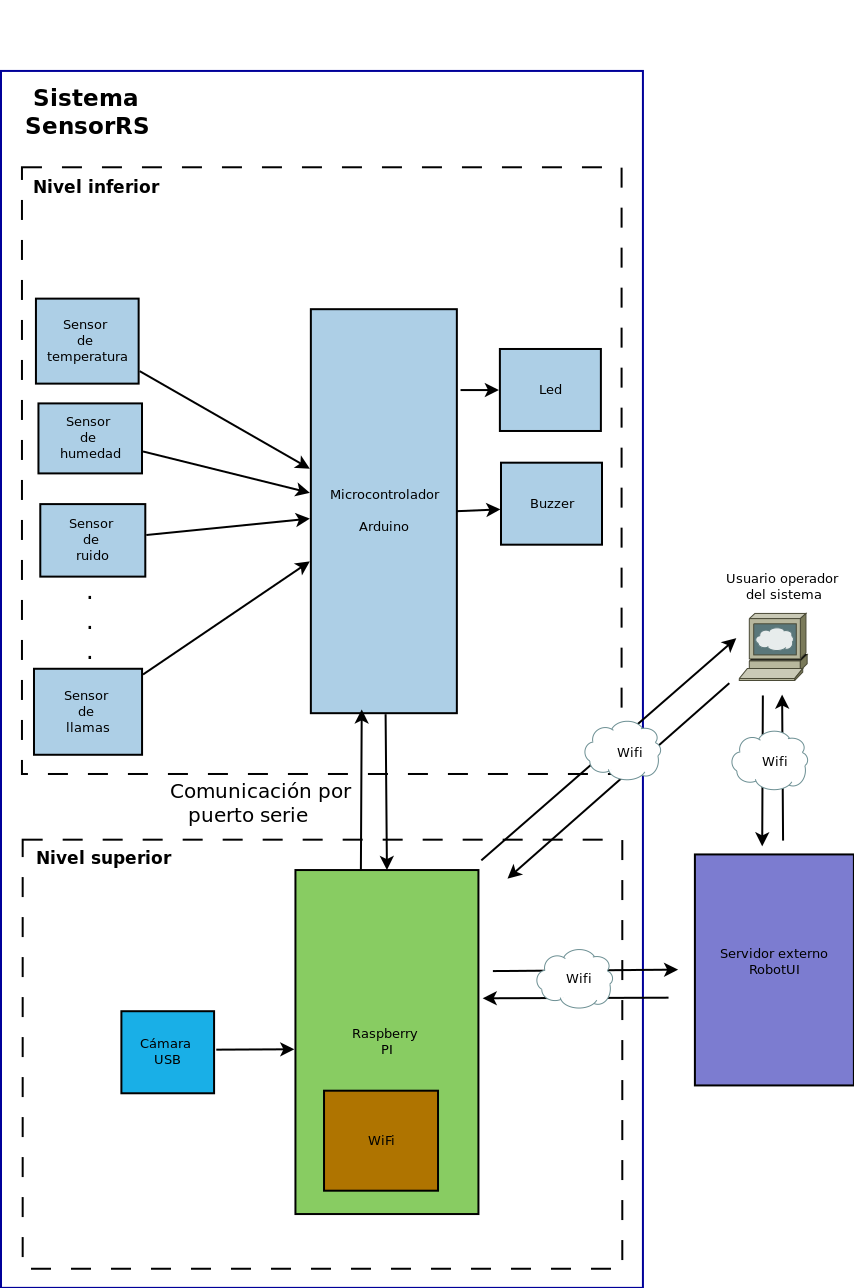
\includegraphics[width=4.0cm]{diagrama_bloques_general.png}
      \end{figure}
     \end{center}
\end{column}
\end{columns}

}


\section{Desarrollo}

\frame{\frametitle{\textcolor{black}{ Subsistemas }}

\begin{figure}[H]
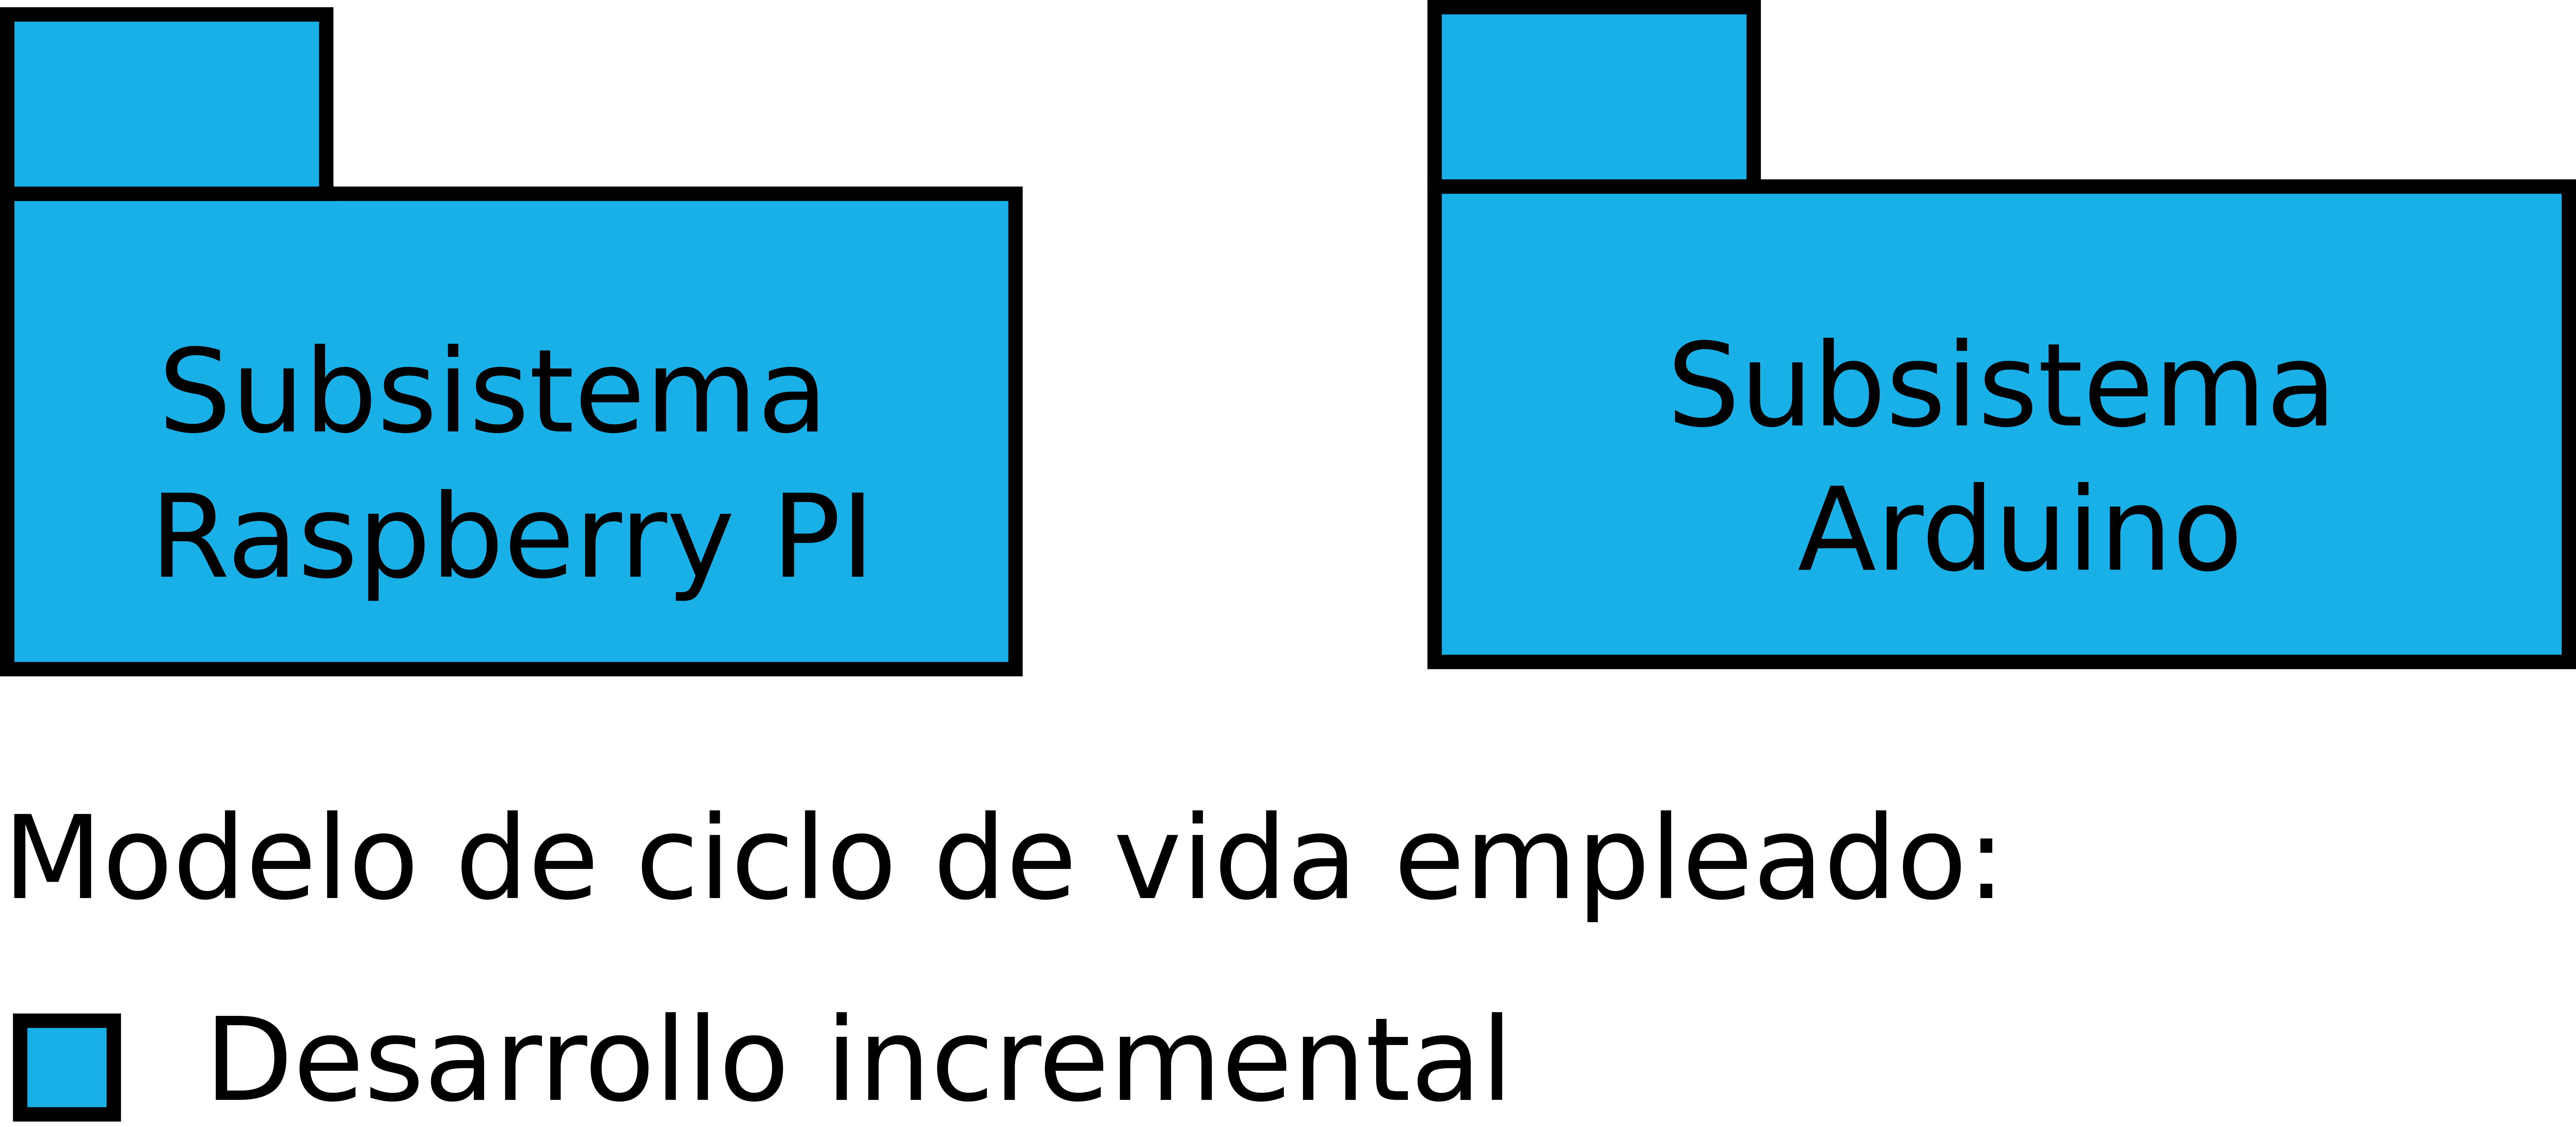
\includegraphics[width=9cm]{subsistemas.png}
\end{figure}

}


\section{Temporización}

\frame{\frametitle{\textcolor{black}{ Temporización }}

\begin{figure}[H]
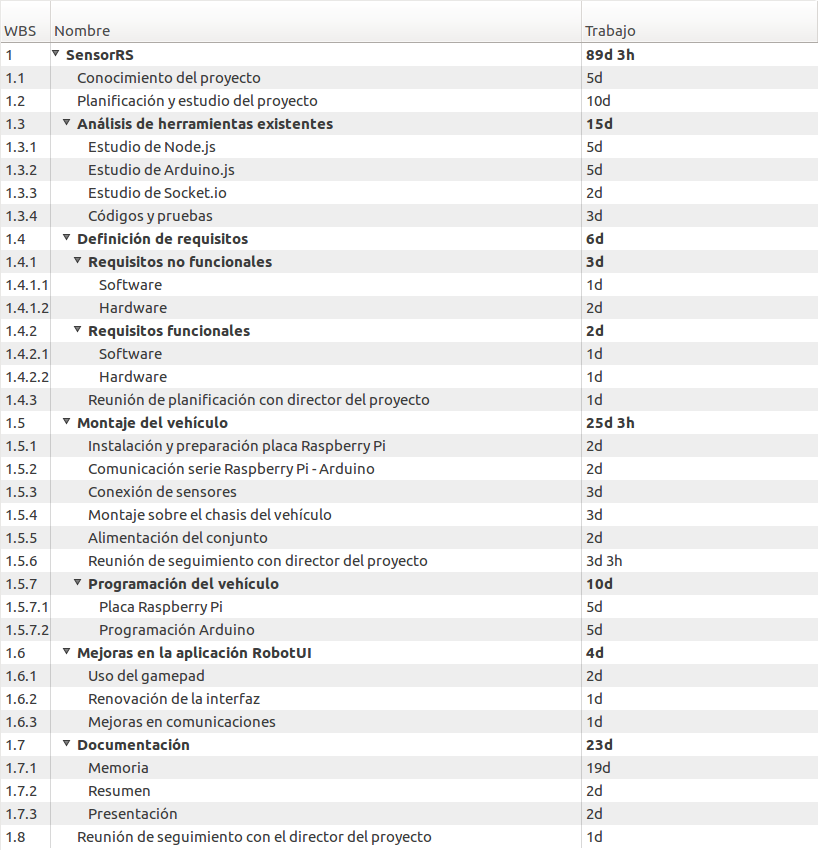
\includegraphics[width=6cm]{planificacion.png}
\end{figure}

}


\frame{\frametitle{\textcolor{black}{ Temporización }}

\begin{adjustwidth}{-2em}{-1em}

\begin{figure}[H]
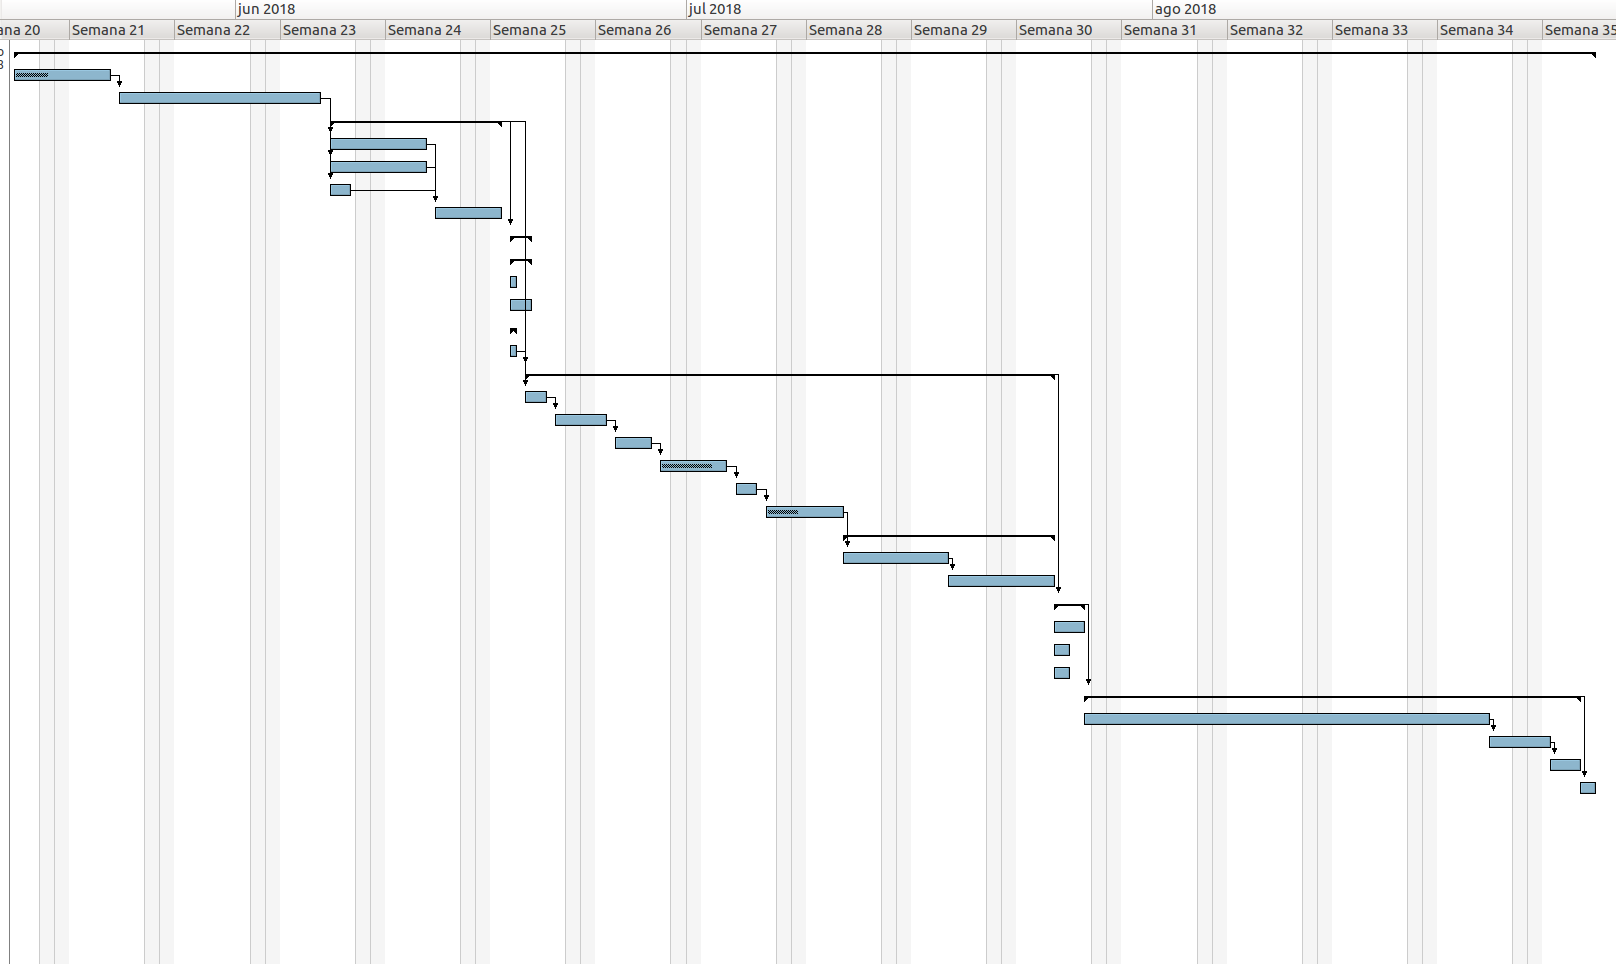
\includegraphics[width=10cm]{gantt_01.png}
\end{figure}

\end{adjustwidth}

}


\section{Herramientas software}

\frametitle{\textcolor{black}{Herramientas software}}

\begin{figure}[H]
  
\includegraphics[width=4cm]{nodejs-logo.png}
\end{figure}

\begin{figure}[H]
  
\includegraphics[width=4cm]{socketio-logo.png}
\end{figure}


\begin{figure}[H]
  
\includegraphics[width=4cm]{ffmpeg-logo.jpg}
\end{figure}

\begin{figure}[H]
  
\includegraphics[width=4cm]{arduino_ide_logo.png}
\end{figure}
}

\section{Herramientas hardware}


\subsection{Raspberry Pi y Arduino}


\begin{frame}[fragile]
\frametitle{\textcolor{black}{Placas utilizadas}}

\begin{figure}%
    \centering
    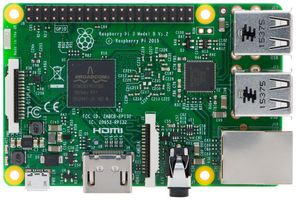
\includegraphics[width=4cm]{raspberry-pi.jpg}
    \qquad
    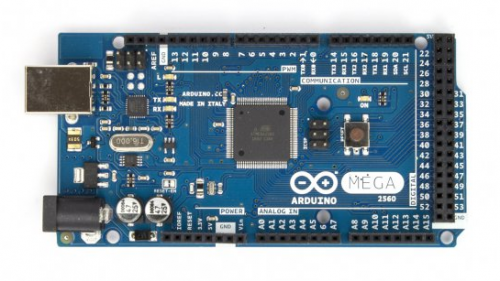
\includegraphics[width=5cm]{arduino.png}
\end{figure}

\begin{center}
  Imagen de una Raspberry Pi (izquierda) y una Arduino Mega (derecha) utilizadas en SensorRS.
\end{center}
 
\end{frame}


\subsection{Complementos hardware}

\begin{frame}[fragile]
\frametitle{\textcolor{black}{ Complementos hardware}}

\begin{columns}
\begin{column}{0.5\textwidth}
\begin{figure}[H]
  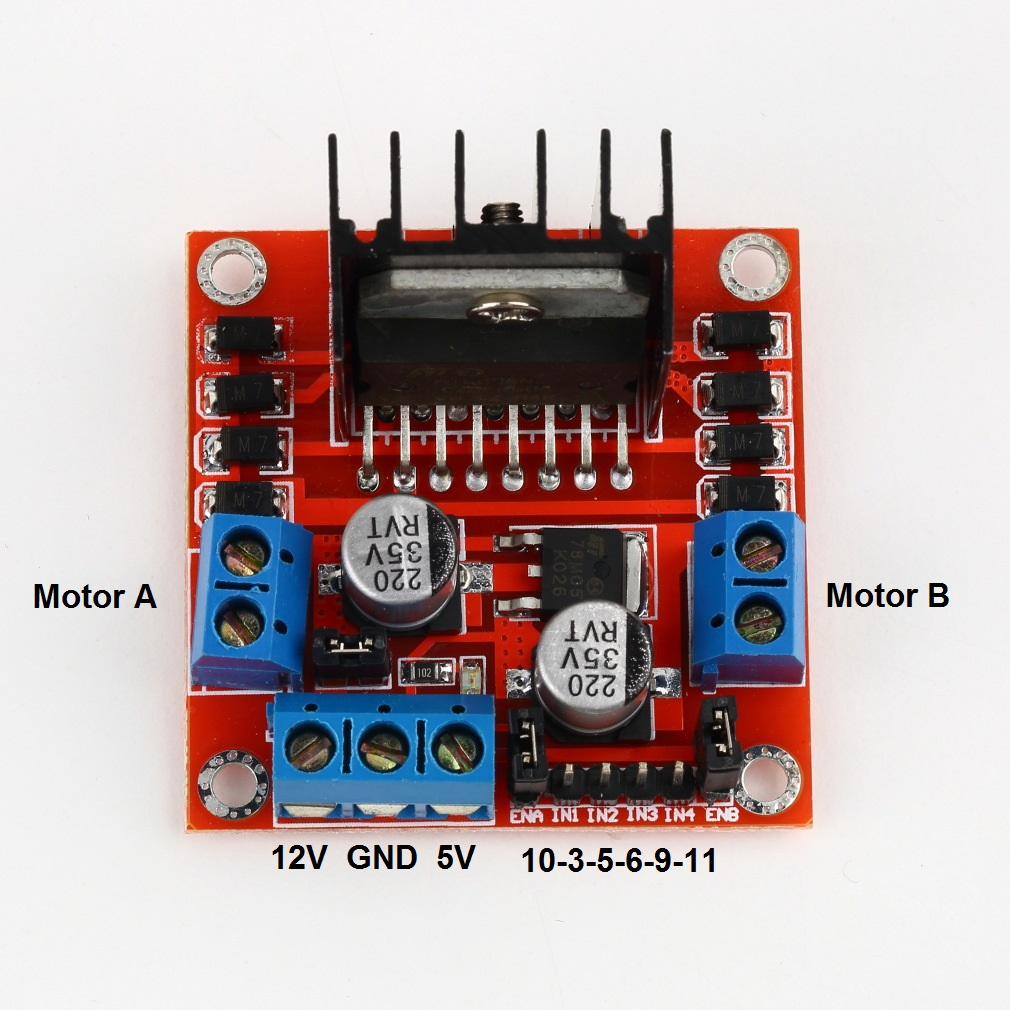
\includegraphics[width=2cm]{l298n.jpg}
\end{figure}
\begin{center}
\caption{Driver de motores L298N.} 
\end{center}

\begin{figure}[H]
  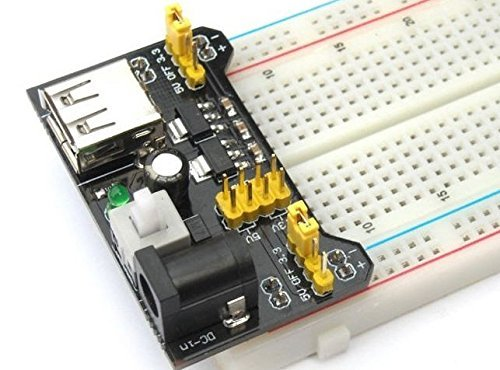
\includegraphics[width=2cm]{alimentador_usb.jpg}
\end{figure}
\begin{center}
\caption{Alimentador USB para protoboard.} 
\end{center}

\end{column}
\begin{column}{0.5\textwidth}
\begin{figure}[H]
  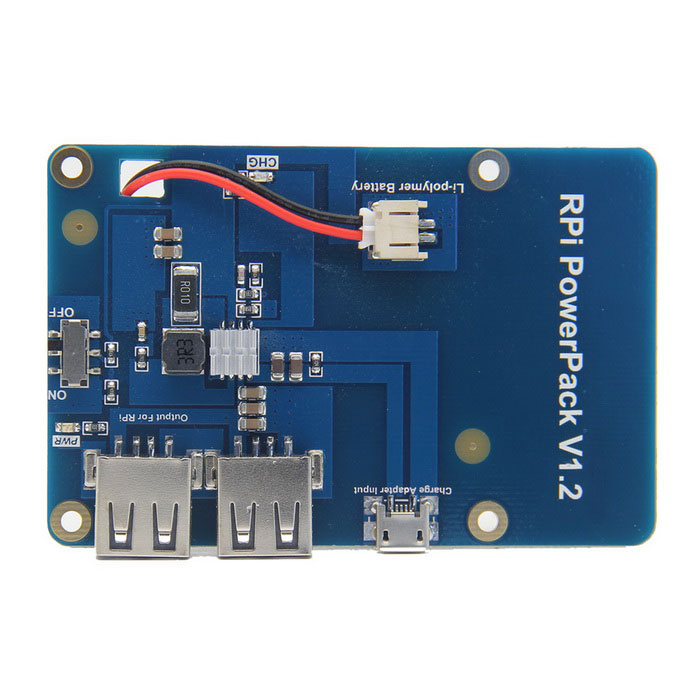
\includegraphics[width=2cm]{modulo-alimentacion.jpg}
\end{figure}
\begin{center}
\caption{Módulo de alimentación para Raspberry Pi.} 
\end{center}

\begin{figure}[H]
  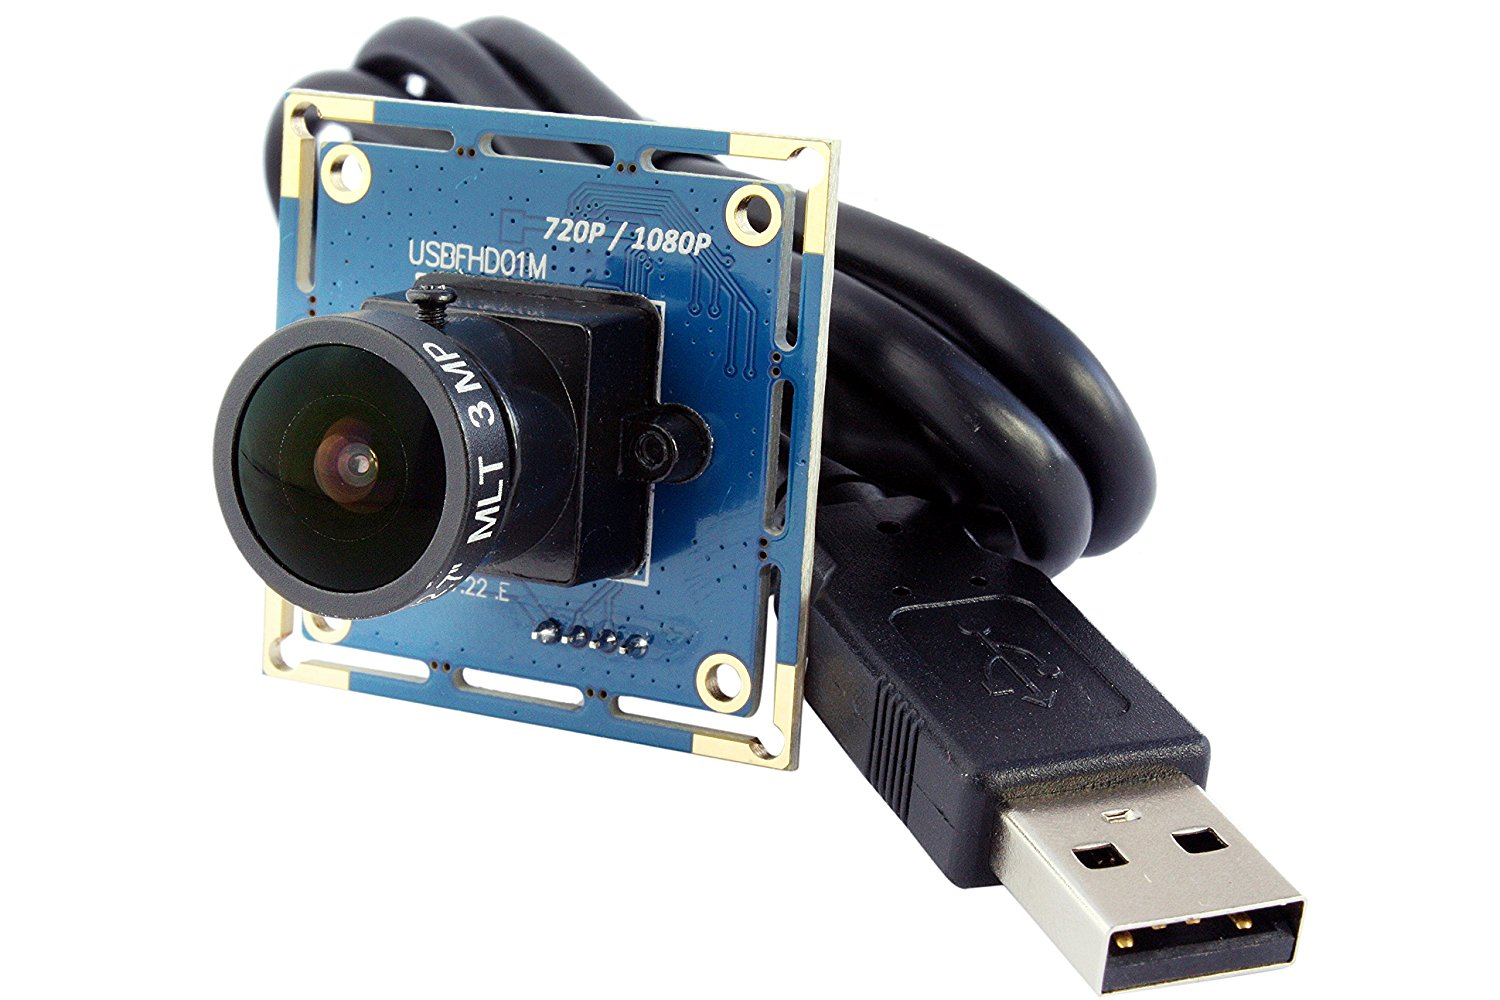
\includegraphics[width=2cm]{camara-usb.jpg}
\end{figure}
\begin{center}
\caption{Cámara USB alta definición.} 
\end{center}
\end{column}
\end{columns}

\end{frame}


\subsection{Sensores}
\frame{\frametitle{\textcolor{black}{ Sensores utilizados }}

\begin{figure}%
    \centering
    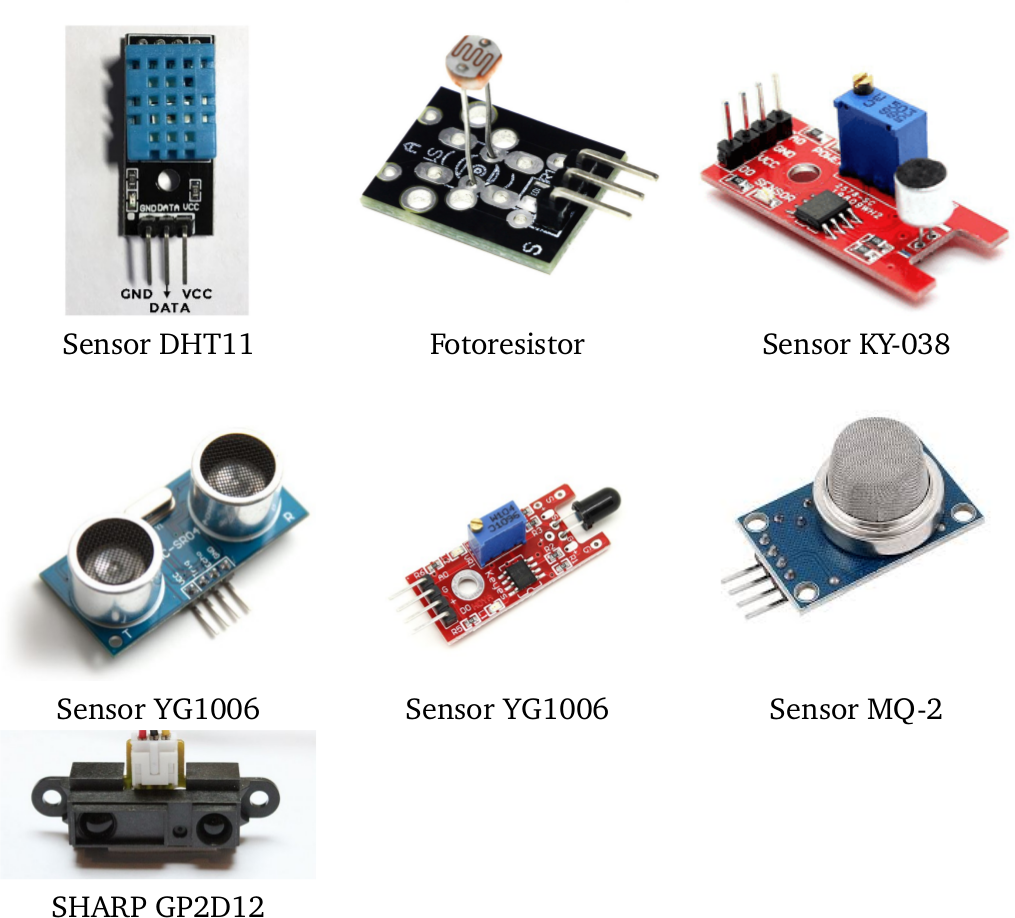
\includegraphics[scale=0.6]{sensores.png}
\end{figure}

\begin{center}
Conjunto de sensores integrados en SensorRS.
\end{center}

}


\section{Esquemático}

\begin{frame}[fragile]
\frametitle{\textcolor{black}{ Conexionado general}}

\begin{figure}%
    \centering
    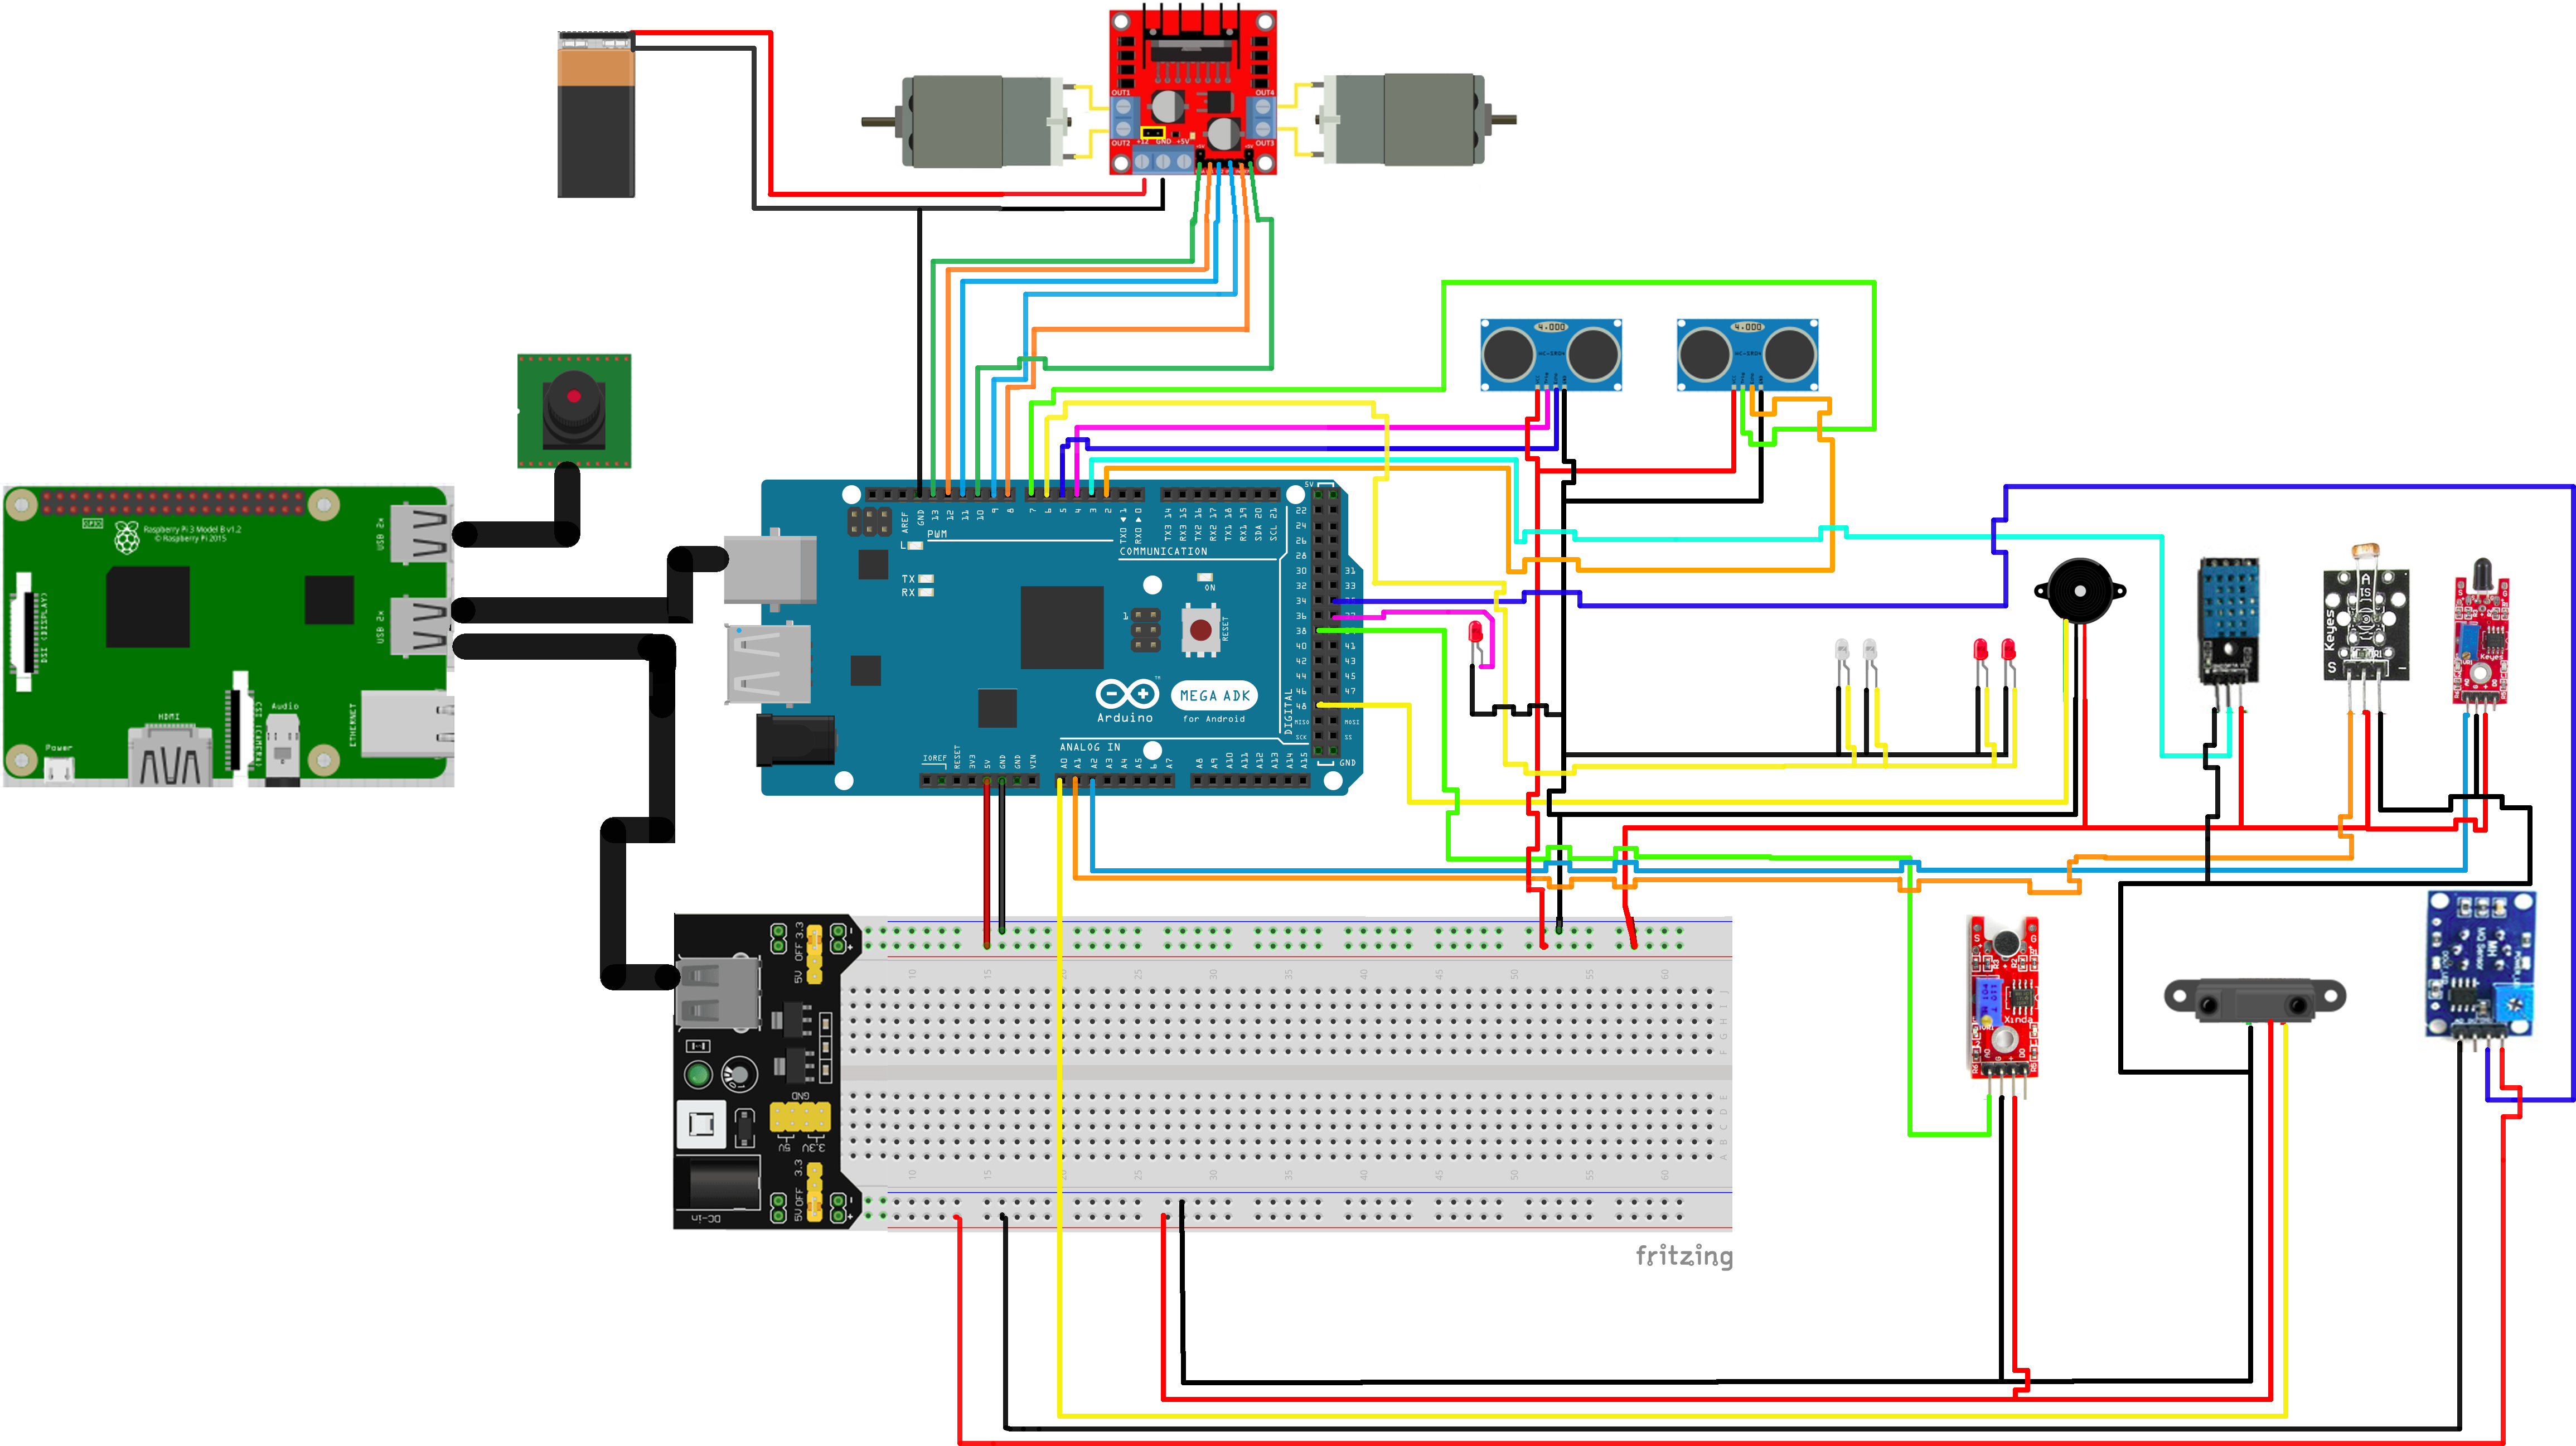
\includegraphics[scale=0.25]{esquema_general.png}
\end{figure}

\begin{center}
Esquemático del conexionado general del robot.
\end{center}

\end{frame}


\section{Esquemático}

\begin{frame}[fragile]
\frametitle{\textcolor{black}{ Conexionado general}}

\begin{figure}%
    \centering
    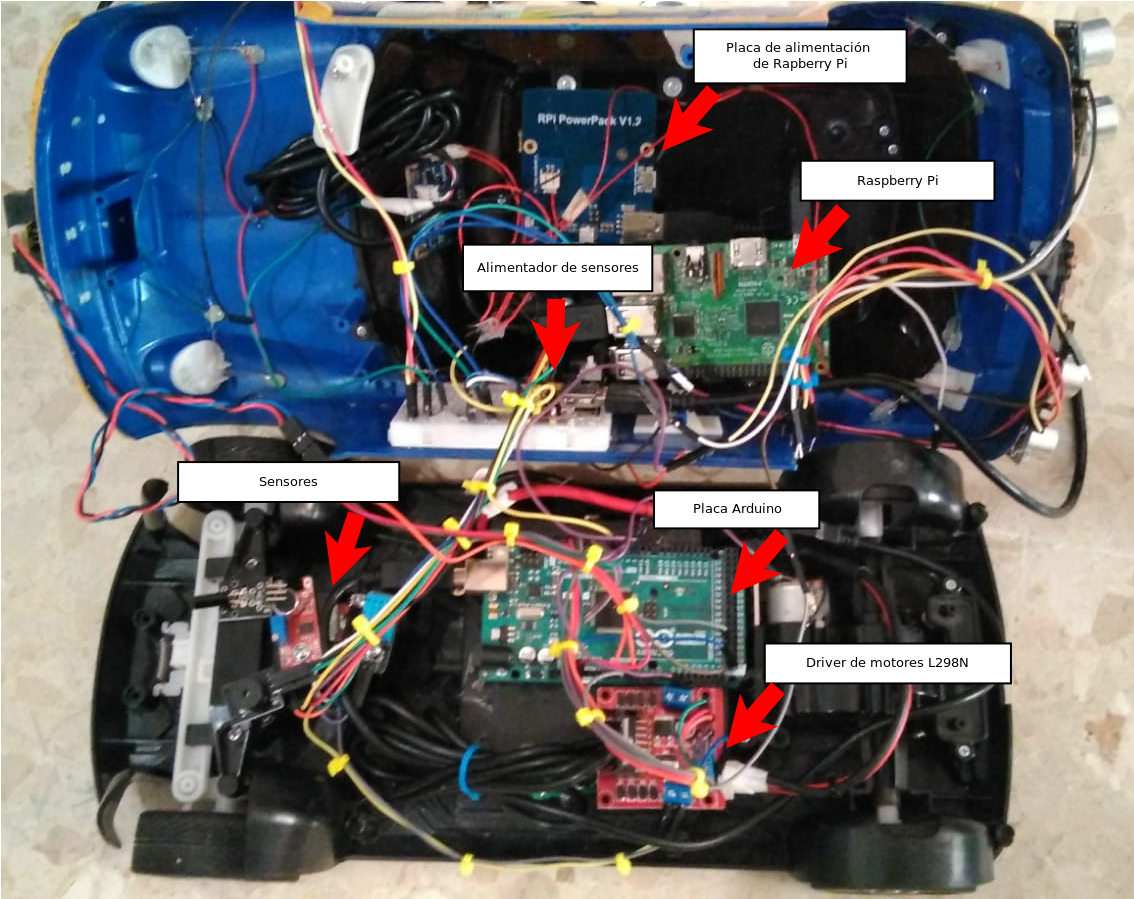
\includegraphics[scale=0.18]{conexionado_etiquetas_general.png}
\end{figure}

\begin{center}
Esquemático del conexionado general del robot.
\end{center}

\end{frame}



\section{Motores}

\begin{frame}[fragile]
\frametitle{\textcolor{black}{ PWM }}

\begin{figure}%
    \centering
    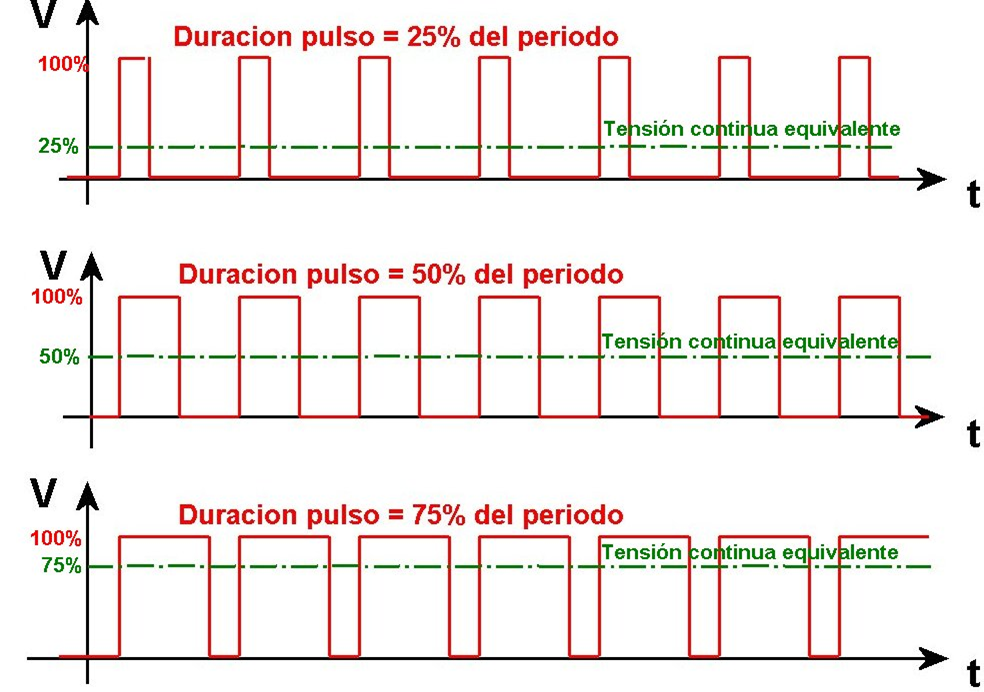
\includegraphics[scale=0.18]{pwm.png}
\end{figure}

\begin{center}
Señales PWM.
\end{center}

\end{frame}


\section{Motores}

\begin{frame}[fragile]
\frametitle{\textcolor{black}{ Control de motores }}

\begin{columns}
\begin{column}{0.4\textwidth}
\begin{figure}[H]
  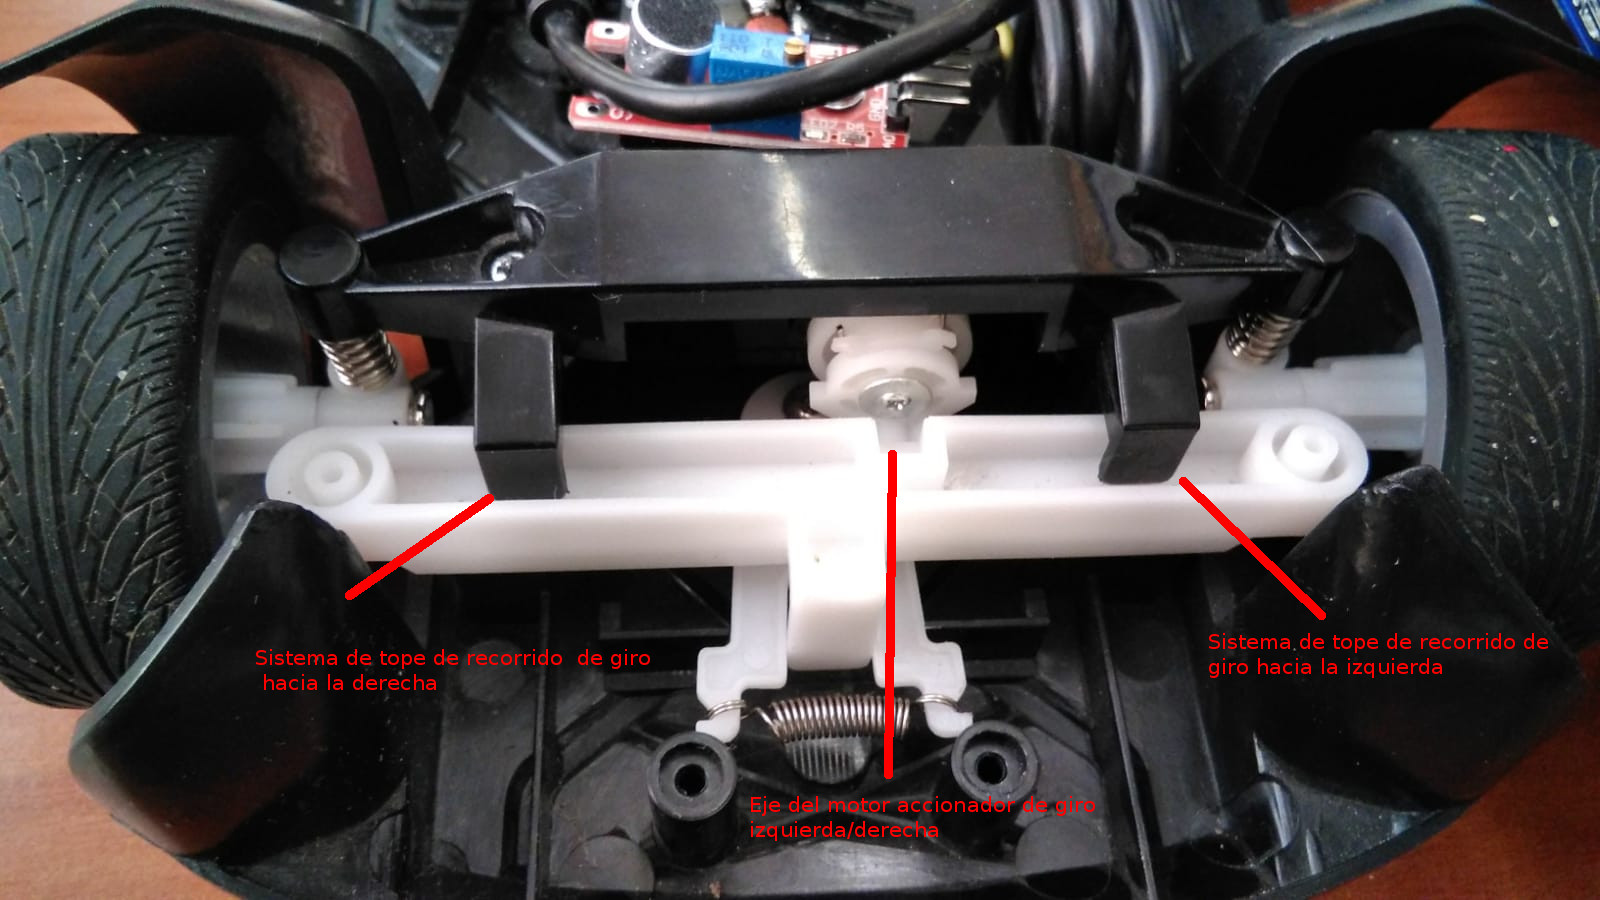
\includegraphics[width=3cm]{motor-direccion.jpg}
\end{figure}
\begin{center}
\caption{Motor de dirección.} 
\end{center}
\end{column}



\begin{column}{0.4\textwidth}
\begin{figure}[H]
  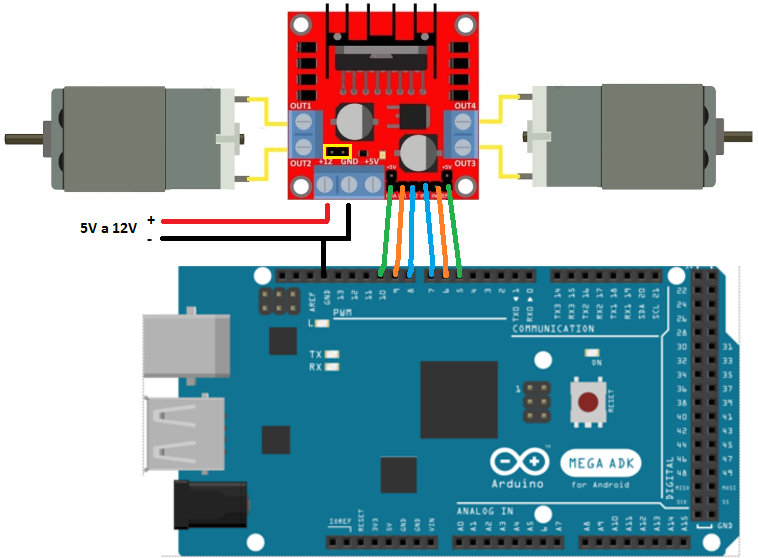
\includegraphics[width=4cm]{L298N_conexionado.png}
\end{figure}
\begin{center}
\caption{Conexionado.} 
\end{center}
\end{column}


\begin{column}{0.4\textwidth}
\begin{figure}[H]
  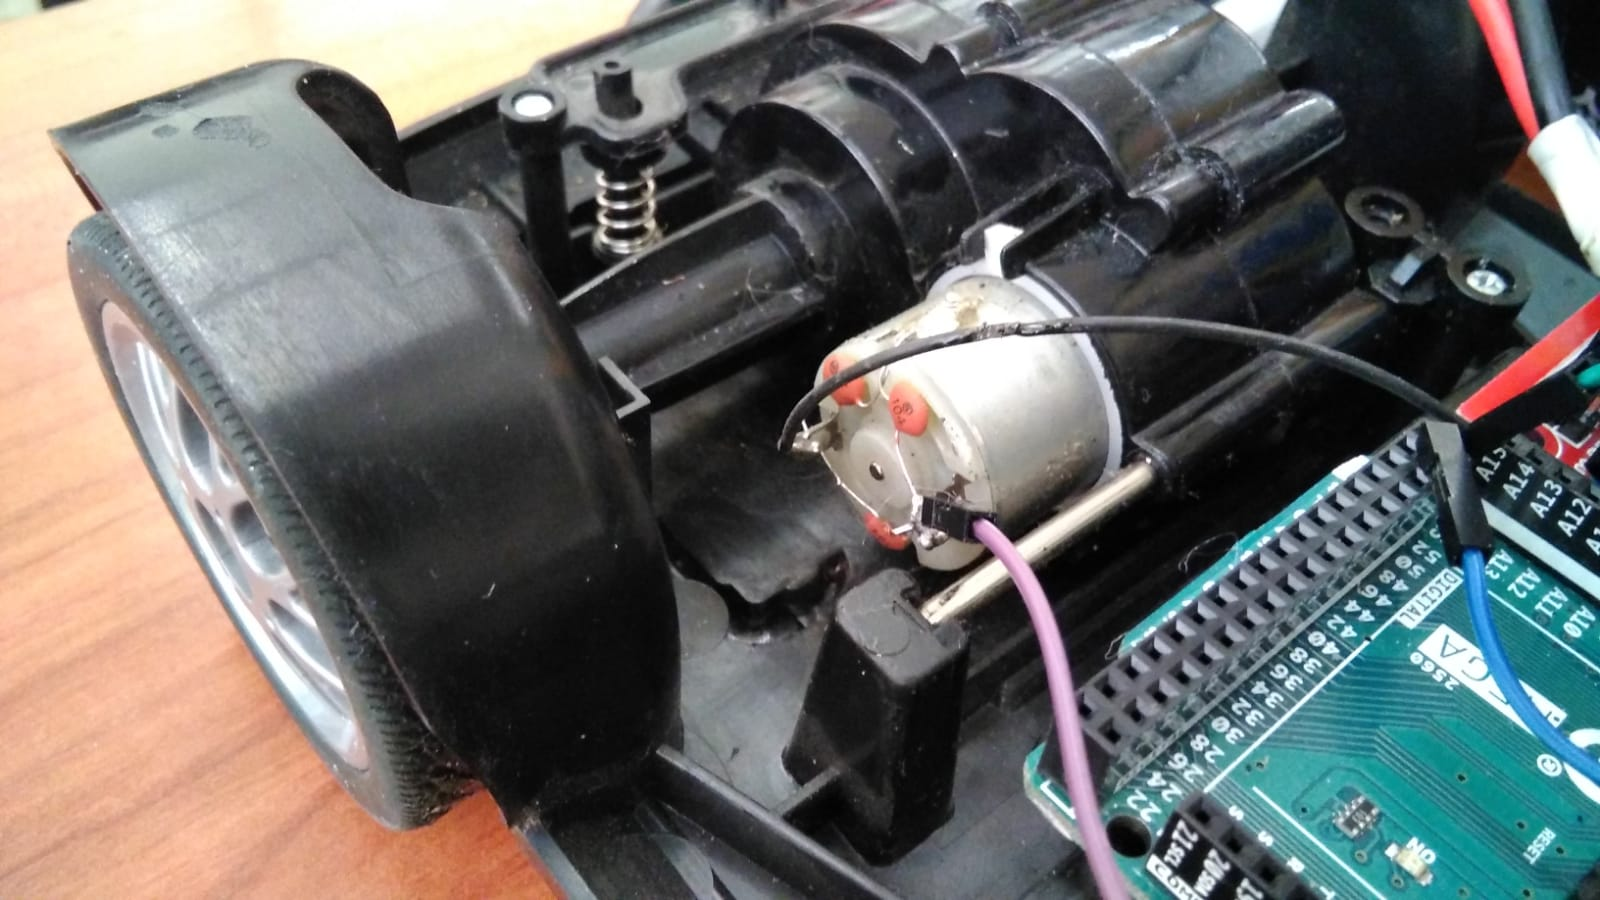
\includegraphics[width=3cm]{motor-traccion.jpg}
\end{figure}
\begin{center}
\caption{Módulo de tracción.} 
\end{center}
\end{column}


\end{columns}

\end{frame}



\section{Comunicaciones}

\begin{frame}[fragile]
\frametitle{\textcolor{black}{ Comunicaciones Serie }}
\textbf{Transmisión de Raspberry Pi a Arduino:}
\begin{lstlisting}[language=JavaScript]
const SerialPort = require ('serialport');
const Readline = SerialPort.parsers.Readline;
const port = new SerialPort('/dev/ttyACM0',{ baudRate: 9600 });
const parser = new Readline();
port.pipe(parser);

function serial_transmission(data,delay){
	setTimeout(function(){
	  //Envío del string caracter por caracter
	  for(vari=0;i<data.length;i++){
	    port.write(newBuffer(data[i],'ascii'));
	  }

	  //Caracter final \n
	  port.write(newBuffer('\n','ascii'));
	},delay);
}

\end{lstlisting}

\end{frame}


\begin{frame}[fragile]
\frametitle{\textcolor{black}{ Comunicaciones Serie }}
\textbf{Captura de mensaje en Raspberry Pi procedente de Arduino:}

  \begin{lstlisting}[language=JavaScript]
  const parser = port.pipe(new Readline({delimiter: '\r\n'}));
  parser.on('data', function(data){
    console.log(data) ;
    var msg_data = data.split("%");
    socket.emit(String(msg_data[0]), { msg: String(msg_data[1]) } );
  }) ;

  \end{lstlisting}
    
  \\  
  Siendo msg\_data[0] el indicativo del tipo de dato y msg\_data[1] su valor
    
\end{frame}



\begin{frame}[fragile]
\frametitle{\textcolor{black}{ Comunicaciones Serie }}
\textbf{Captura de mensaje en Arduino procedente de Raspberry Pi:}
\begin{lstlisting}[language=JavaScript]
void loop(){
  while(Serial.available()>0){
  charreceived=Serial.read();
  inData.concat(received);
  if(received==’\n’){
    inData.trim();
    //MOTOR
    if(inData.startsWith("MOTOR")){
      if(sscanf(inData.c_str(),"MOTOR-%d",&motor)==1){
	Serial.println(motor);
      }
      if(motor<=51 && motor >= -51 ){
	Serial.println ('STOP');
      }
    }
    inData="";
  }
 delay(100);
}
\end{lstlisting}

\end{frame}



\begin{frame}[fragile]
\frametitle{\textcolor{black}{ Comunicaciones Serie }}
\textbf{Envío de mensaje a Raspberry Pi procedente de Arduino:}

\begin{lstlisting}[language=JavaScript]
void loop(){
	bytetemperature=0;
	bytehumidity=0;
	interr=SimpleDHTErrSuccess;
	if((err=dht11.read(pinDHT11,&temperature,&humidity,NULL)) != SimpleDHTErrSuccess){
			Serial.print("ReadDHT11failed,err=");
			Serial.println(err);delay(1000);
		}
	dht11.read(pinDHT11,&temperature,&humidity,NULL);
	
	if((int)temperature!=0and(int)humidity!=0){
		Serial.print("tmp%");
		Serial.print((int)temperature);Serial.print("*C,");
		Serial.print((int)humidity);Serial.println("H");
	}

	delay(30);
	Serial.println(analogRead(photosensorPin));
}
\end{lstlisting}
\end{frame}



\section{Conclusiones}

\frame{\frametitle{\textcolor{black}{Conclusiones}}
  La realización del trabajo \emph{SensorRS: Asistente de diseño de interfaz de control, seguimiento y sharing de
robots en tiempo real} como trabajo de fin de carrera, se ha caracterizado por:

\begin{itemize}
    \item La elaboración de un vehículo robótico haciendo uso de una Raspberry Pi 3 Model B.
    \item Programación del microcontrolador Atmega2560 alojado en una placa Arduino.
    \item Comunicación por puerto serie entre la placa Arduino y Raspberry Pi
    \item Realización de conexiones entre elementos y montaje del vehículo.
    \item Transmisión de gran cantidad de datos entre cliente servidor y servidor cliente. Streaming de vídeo y audio, emisión de comandos entre otros datos.     
\end{itemize}

}


\section{Referencias}
 
\begin{thebibliography}{8}
\beamertemplatebookbibitems 

\bibitem{article:4}\color{black}
Hau-Shiue Juang and Kai-Yew Lum.
\newblock {Design and Control of a Two-Wheel Self-Balancing Robot using the
  Arduino Microcontroller Board}.\color{black}
\newblock {\color{black} Technical report, IEEE International Conference on Control and
  Automation, 5 2013}.

\bibitem{book:Sensors}\color{black}
{Kimmo Karvinen & Tero Karvinen}.
\newblock {\em Make: Getting Started with Sensors}.\color{black}
\newblock { \color{black} Make Media Books, 2014.}

\bibitem{article:5}\color{black}
Nilson~Mori Lazarin and Carlos~Eduardo Pantoja.
\newblock {A Robotic-agent Platform For Embedding Software Agents usin
  Raspberry Pi and Arduino Boards}.\color{black}
\newblock {\color{black} Technical report, UnED Nova Friburgo, 6 2011.}

\bibitem{book:sensoresyactuadores}\color{black}
{Leonel G. Corona Ramírez & Griselda S. Abarca Jiménez & Jesús Mares
  Carreño}.
\newblock {\em Sensores y actuadores, Aplicaciones con Arduino}.\color{black}
\newblock {\color{black} Grupo Editorial Patria, 2014.\}

\bibitem{book:pwm}\color{black}
D.~Grahame Holmes & Thomas~A. Lipo.
\newblock {\em Pulse Width Modulation for Power Converters}.\color{black}
\newblock {\color{black} Power Engineering, 2012.}


\bibitem{article:2}\color{black}
Lakshminarasimhan Srinivasan, Julian Scharnagl, and Klaus Schilling.
\newblock {Analysis of WebSockets as the New Age Protocol for Remote Robot
  Tele-operation}.\color{black}
\newblock { \color{black}Technical report, University of Wuerzburg, Department of Robotics and
  Telematics, 11 2013.}

\bibitem{article:1}\color{black}
Lakshminarasimhan Srinivasan, Julian Scharnagl, Zhihao Xu, Nicolas Faerber,
  Dinesh~K. Babu, and Klaus Schilling.
\newblock {Design and Development of a Robotic Teleoperation System using
  Duplex WebSockets suitable for Variable Bandwidth Networks}\color{black}.
\newblock{\color{black} Technical report, University of Wuerzburg, Department of Robotics and
  Telematics, 11 2013.}


\bibitem{article:3}\color{black}
Nazirah~Ahmad Zaini, Norliza Zaini, Mohd Fuad~Abdul Latip, and Nabilah Hamzah.
\newblock {Remote Monitoring System based on a Wi-Fi Controlled Car Using
  Raspberry Pi}.\color{black}
\newblock { \color{black} Technical report, Universiti Teknologi MARA (UiTM) Shah Alam,
  Malaysia, Faculty of Electrical Engineering, 12 2016.}

\end{thebibliography}



\begin{frame}[label=firstframe]
    \titlepage % (Or whatever else goes here.)
\end{frame}

\end{document}




